\documentclass[a4paper]{article}

\usepackage[utf8]{inputenc}
\PassOptionsToPackage{hyphens}{url} % zodat url's ook afgekapt worden
\usepackage{hyperref}
\usepackage[dutch]{babel}
\usepackage{graphicx}
\usepackage{algorithm}
\usepackage{algorithmic}
\usepackage{mathtools}
\usepackage{tikz}
\usepackage{tocbibind}
\usepackage{float}
\usepackage{framed}
\usepackage{parskip}
\usepackage{listings}
\usepackage{color}
\usepackage{pdfpages}
\usepackage{pdflscape}
\usepackage{todonotes}

\title{Software Engineering Analyse: \\ Restaurant Management Systeem}
\author{Vincent Drozdzyniak 1334231 \\ Hendrik Lievens 1130921 \\ Martijn Maes 1131102 \\ Reinaert Van de Cruys 1334947 \\ Michiel Vanmunster 1334724 \\ Jens Vannitsen 1334039}
\date{3 maart 2016}

\begin{document}
\maketitle


\section{Probleemstelling}
Het opvolgen van reserveringen, bestellingen, tafels en rekeningen kan in grote restaurants een probleem vormen. Klanten die willen reserveren moeten bellen, in de hoop dat er nog een plaats vrij is. Ook is het Voor het zaalpersoneel het niet altijd eenvoudig om elke tafel een gelijkwaardige hoevelheid service te bieden en moeten klanten op een druk moment lang wachten om een bestelling te doen of een rekening op te vragen.

Er bestaan reeds verschillende systemen om restaurantuitbaters hierin te ondersteunen, zoals  \textit{lightspeedhq.be} of \textit{lsretail.com}. De focus van deze systemen ligt voornamelijk op het beheren van de inventaris, het onderhouden van een leveranciersdatabase, het beheren van het personeel, \dots

Om deze problemen aan te kaarten, ontwikkelen wij een softwarepakket dat het personeel bijstaat en hun werk vergemakkelijkt. Klanten kunnen via een eenvoudige, \textit{responsive}, web-interface reserveringen maken, dranken en gerechten bestellen, een rekening vragen, \dots Het zaalpersoneel krijgt een duidelijk overzicht van elke tafel en kan zo zien waar er nood is aan bediening en bestellingen opvolgen. 

\clearpage
\section{Requirements analyse} 
De functionele requirements zijn:
\begin{enumerate}
\item Het systeem laat meerdere gebruikersrollen toe:
\begin{enumerate}
\item De beheerder / uitbater
\item Personeelsleden
\item Klanten
\end{enumerate}
\item De uitbater kan het vloerplan van zijn zaak opstellen, opslaan en wijzigen.
\item De uitbater kan personeel beheren en functies toekennen.
\item Het personeel kan reservaties beheren.
\item Het personeel kan menu's beheren.
\item Het personeel kan bestellingen beheren.
\item Het personeel kan een rekening laten opmaken.
\item Het personeel kan voorraad beheren.
\item Het personeel kan een overzicht bekijken van de tafels.
\item Het personeel kan raadplegen hoe lang klanten reeds aan het wachten zijn.
\item Het personeel kan een overzicht bekijken van lopende bestellingen.
\item Een klant moet een reservatie kunnen maken aan de hand van een kalender.
\item Een klant kan een vrije tafel kiezen bij het reserveren.
\item Een klant moet de menu kaart kunnen bekijken op zijn smartphone / tablet.
\item Een klant moet, zonder hulp van een ober, een gerecht kunnen bestellen.
\item Een klant moet, zonder hulp van een ober, een drankje kunnen bestellen.
\item Een klant moet een ober kunnen roepen.
\item Een klant moet zijn rekening kunnen opvragen.
\end{enumerate}
\section{URPS} 
\subsection{Usability}
Gebruiksvriendelijkheid is een belangrijk aspect van dit project. Klanten moeten op een eenvoudige manier kunnen reserven en een bestelling plaatsen. Zaal- en keukenpersoneel moet een duidelijk overzicht hebben van de zaal en van de lopende bestellingen. Het systeem moet een ontspannende avond op restaurant ondersteunen met zijn gebruiksgemak.
\subsection{Reliability}
Het platform moet enorm betrouwbaar zijn. Een crash kan nefast zijn wanneer er veel bestellingen lopen en de klanten blijven toestromen. Wanneer een client crasht, blijft alle data bewaard op de server. Wanneer de server crasht, moet het personeel deze herstarten en tijdelijk vertrouwen op de lokale kopies van clients. 
\subsection{Performance}
Door gebruik te maken van een client-server model, kunnen we ook performantie optimaliseren. Meerdere clients (computers van klanten thuis, tablets in het restaurant, \dots) staan in verbinding met de server, die het rekenwerk voor zich neemt en de clients controleert.
Het maken van reservaties, plaatsen van bestellingen, \dots moeten responsief aanvoelen, met minimale vertraging. 
\subsection{Supportability}
Het systeem moet op een eenvoudige manier uitbreidbaar en onderhoudbaar zijn. Dit wordt ondersteund door het werken met verschillende modules om zo de noden van klant tot klant te kunnen invullen. Door specifieke aanvragen van klanten om te vormen tot modules, kunnen op een later tijdstip deze modules hergebruikt worden. Indien de wetgeving rond horeca zou wijzigen, moet het systeem snel aan te passen zijn.
\subsection{Legal}
Het systeem moet conform zijn met de bestaande wetgeving voor de horeca en correct omspringen met de privacy van klanten en personeel.

\section{Kost}
We schatten zo'n 30 dagen per persoon nodig te hebben, dit komt neer op zo'n 180 werkdagen.

\section{Mockups}
\begin{figure}[H]
\centering
  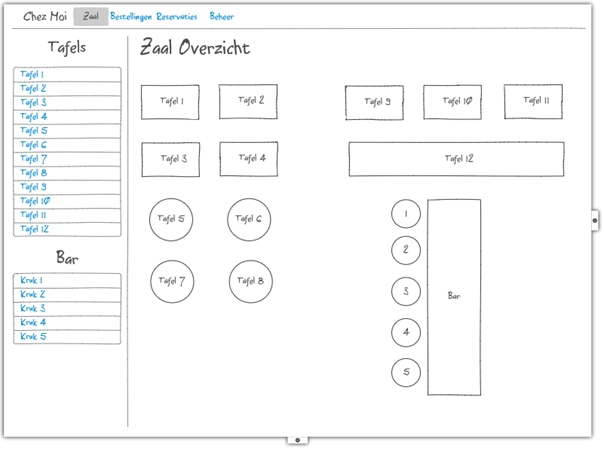
\includegraphics[width=1.0\linewidth]{restaurant_mockup.jpg}
\end{figure}


\end{document}